\documentclass{ximera}

%\usepackage{todonotes}

\newcommand{\todo}{}

\usepackage{tkz-euclide}
\tikzset{>=stealth} %% cool arrow head
\tikzset{shorten <>/.style={ shorten >=#1, shorten <=#1 } } %% allows shorter vectors

\usepackage{tkz-tab}  %% sign charts
\usetikzlibrary{decorations.pathreplacing} 

\usetikzlibrary{backgrounds} %% for boxes around graphs
\usetikzlibrary{shapes,positioning}  %% Clouds and stars
\usetikzlibrary{matrix} %% for matrix
\usepgfplotslibrary{polar} %% for polar plots
\usetkzobj{all}
\usepackage[makeroom]{cancel} %% for strike outs
%\usepackage{mathtools} %% for pretty underbrace % Breaks Ximera
\usepackage{multicol}

\usepackage{polynom}



\usepackage[many]{tcolorbox}  %% for titled boxes
\newtcolorbox{xbox}[1]{%
    tikznode boxed title,
    enhanced,
    arc=0mm,
    interior style={white},
    attach boxed title to top center= {yshift=-\tcboxedtitleheight/2},
    fonttitle=\bfseries,
    colbacktitle=white,coltitle=black,
    boxed title style={size=normal,colframe=white,boxrule=0pt},
    title={#1}}


\usepackage{array}
\setlength{\extrarowheight}{+.1cm}   
\newdimen\digitwidth
\settowidth\digitwidth{9}
\def\divrule#1#2{
\noalign{\moveright#1\digitwidth
\vbox{\hrule width#2\digitwidth}}}





\newcommand{\RR}{\mathbb R}
\newcommand{\R}{\mathbb R}
\newcommand{\N}{\mathbb N}
\newcommand{\Z}{\mathbb Z}

%\renewcommand{\d}{\,d\!}
\renewcommand{\d}{\mathop{}\!d}
\newcommand{\dd}[2][]{\frac{\d #1}{\d #2}}
\newcommand{\pp}[2][]{\frac{\partial #1}{\partial #2}}
\renewcommand{\l}{\ell}
\newcommand{\ddx}{\frac{d}{\d x}}
\newcommand{\ddt}{\frac{d}{\d t}}

\newcommand{\zeroOverZero}{\ensuremath{\boldsymbol{\tfrac{0}{0}}}}
\newcommand{\inftyOverInfty}{\ensuremath{\boldsymbol{\tfrac{\infty}{\infty}}}}
\newcommand{\zeroOverInfty}{\ensuremath{\boldsymbol{\tfrac{0}{\infty}}}}
\newcommand{\zeroTimesInfty}{\ensuremath{\small\boldsymbol{0\cdot \infty}}}
\newcommand{\inftyMinusInfty}{\ensuremath{\small\boldsymbol{\infty - \infty}}}
\newcommand{\oneToInfty}{\ensuremath{\boldsymbol{1^\infty}}}
\newcommand{\zeroToZero}{\ensuremath{\boldsymbol{0^0}}}
\newcommand{\inftyToZero}{\ensuremath{\boldsymbol{\infty^0}}}



\newcommand{\numOverZero}{\ensuremath{\boldsymbol{\tfrac{\#}{0}}}}
\newcommand{\dfn}{\textbf}
%\newcommand{\unit}{\,\mathrm}
\newcommand{\unit}{\mathop{}\!\mathrm}
\newcommand{\eval}[1]{\bigg[ #1 \bigg]}
\newcommand{\seq}[1]{\left( #1 \right)}
\renewcommand{\epsilon}{\varepsilon}
\renewcommand{\iff}{\Leftrightarrow}

\DeclareMathOperator{\arccot}{arccot}
\DeclareMathOperator{\arcsec}{arcsec}
\DeclareMathOperator{\arccsc}{arccsc}
\DeclareMathOperator{\si}{Si}
\DeclareMathOperator{\proj}{proj}
\DeclareMathOperator{\scal}{scal}


\newcommand{\tightoverset}[2]{% for arrow vec
  \mathop{#2}\limits^{\vbox to -.5ex{\kern-0.75ex\hbox{$#1$}\vss}}}
\newcommand{\arrowvec}[1]{\tightoverset{\scriptstyle\rightharpoonup}{#1}}
\renewcommand{\vec}{\mathbf}
\newcommand{\veci}{\vec{i}}
\newcommand{\vecj}{\vec{j}}
\newcommand{\veck}{\vec{k}}
\newcommand{\vecl}{\boldsymbol{\l}}

\newcommand{\dotp}{\bullet}
\newcommand{\cross}{\boldsymbol\times}
\newcommand{\grad}{\boldsymbol\nabla}
\newcommand{\divergence}{\grad\dotp}
\newcommand{\curl}{\grad\cross}
%\DeclareMathOperator{\divergence}{divergence}
%\DeclareMathOperator{\curl}[1]{\grad\cross #1}


\colorlet{textColor}{black} 
\colorlet{background}{white}
\colorlet{penColor}{blue!50!black} % Color of a curve in a plot
\colorlet{penColor2}{red!50!black}% Color of a curve in a plot
\colorlet{penColor3}{red!50!blue} % Color of a curve in a plot
\colorlet{penColor4}{green!50!black} % Color of a curve in a plot
\colorlet{penColor5}{orange!80!black} % Color of a curve in a plot
\colorlet{fill1}{penColor!20} % Color of fill in a plot
\colorlet{fill2}{penColor2!20} % Color of fill in a plot
\colorlet{fillp}{fill1} % Color of positive area
\colorlet{filln}{penColor2!20} % Color of negative area
\colorlet{fill3}{penColor3!20} % Fill
\colorlet{fill4}{penColor4!20} % Fill
\colorlet{fill5}{penColor5!20} % Fill
\colorlet{gridColor}{gray!50} % Color of grid in a plot

\newcommand{\surfaceColor}{violet}
\newcommand{\surfaceColorTwo}{redyellow}
\newcommand{\sliceColor}{greenyellow}




\pgfmathdeclarefunction{gauss}{2}{% gives gaussian
  \pgfmathparse{1/(#2*sqrt(2*pi))*exp(-((x-#1)^2)/(2*#2^2))}%
}


%%%%%%%%%%%%%
%% Vectors
%%%%%%%%%%%%%

%% Simple horiz vectors
\renewcommand{\vector}[1]{\left\langle #1\right\rangle}


%% %% Complex Horiz Vectors with angle brackets
%% \makeatletter
%% \renewcommand{\vector}[2][ , ]{\left\langle%
%%   \def\nextitem{\def\nextitem{#1}}%
%%   \@for \el:=#2\do{\nextitem\el}\right\rangle%
%% }
%% \makeatother

%% %% Vertical Vectors
%% \def\vector#1{\begin{bmatrix}\vecListA#1,,\end{bmatrix}}
%% \def\vecListA#1,{\if,#1,\else #1\cr \expandafter \vecListA \fi}

%%%%%%%%%%%%%
%% End of vectors
%%%%%%%%%%%%%

%\newcommand{\fullwidth}{}
%\newcommand{\normalwidth}{}



%% makes a snazzy t-chart for evaluating functions
%\newenvironment{tchart}{\rowcolors{2}{}{background!90!textColor}\array}{\endarray}

%%This is to help with formatting on future title pages.
\newenvironment{sectionOutcomes}{}{} 



%% Flowchart stuff
%\tikzstyle{startstop} = [rectangle, rounded corners, minimum width=3cm, minimum height=1cm,text centered, draw=black]
%\tikzstyle{question} = [rectangle, minimum width=3cm, minimum height=1cm, text centered, draw=black]
%\tikzstyle{decision} = [trapezium, trapezium left angle=70, trapezium right angle=110, minimum width=3cm, minimum height=1cm, text centered, draw=black]
%\tikzstyle{question} = [rectangle, rounded corners, minimum width=3cm, minimum height=1cm,text centered, draw=black]
%\tikzstyle{process} = [rectangle, minimum width=3cm, minimum height=1cm, text centered, draw=black]
%\tikzstyle{decision} = [trapezium, trapezium left angle=70, trapezium right angle=110, minimum width=3cm, minimum height=1cm, text centered, draw=black]


\outcome{To be able to use the method of substitution to solve some ``simple'' integrals, with an emphasis on being able to correctly identify what to substitute for.}
\outcome{Undo the Chain Rule.}
\outcome{Calculate indefinite integrals (antiderivatives) using basic substitution.}
\outcome{Calculate definite integrals using basic substitution.}
\title[Dig-In:]{The idea of substitution}
\begin{document}
\begin{abstract}
  We learn a new technique, called substitution, to help us solve
  problems involving integration.
\end{abstract}
\maketitle


Computing antiderivatives is not as easy as computing derivatives.
One issue is that the chain rule can be difficult to ``undo.''  We
have a general method called ``integration by substitution'' that will
somewhat help with this difficulty. 

If the functions are differentiable, we can apply the chain rule and obtain
\[
\ddx f(g(x)) = f'(g(x))g'(x)
\]
If the derivatives are continuous, we can use this equality to evaluate a definite integral. Namely,
\begin{align*}
  \int_a^b f'(g(x))g'(x) \d x &= \eval{f(g(x))}_a^b \\
  &= f(g(b)) - f(g(a)). \\
 \end{align*}
On the other hand, it is also true that
\begin{align*}
  \int_{g(a)}^{g(b)} f'(u)\d u &= \eval{f(u)}_{g(a)}^{g(b)}\\
  &= f(g(b)) - f(g(a)). \\
 \end{align*}
 Since the right hand sides of these equalities are equal,  the left hand sides must be equal, too. So, it follows that
 
\[
  \int_a^b f'(g(x))g'(x) \d x =  \int_{g(a)}^{g(b)} f'(u)\d u .
\]

 
This simple observation  leads to the following theorem. 


\begin{theorem}[Integral Substitution Formula]\index{integral substitution formula} 
Let $g'$ be the derivative of a  function $g$ and let $f'$ be the derivative of a function $f$. If $g'$ is continuous on the interval $[a,b]$ and  $f'$ is
continuous on the interval $[g(a),g(b)]$, then
\[
\int_a^b f'(g(x)) g'(x) \d x =\int_{g(a)}^{g(b)} f'(u) \d u.
\]
\end{theorem}
The integral on the right appears to be much simpler than the original integral.
So, when evaluating a difficult integral,  we try to apply this theorem and replace the original integral with a simpler one.
 We can do this as long as the conditions of the theorem are satisfied.

We will apply the Integral Substitution Formula (ISF)  to the following example.

\begin{example}
Compute:
\[
\int_0^2 x e^{x^2}\d x
\]
\begin{explanation}
Why do we think that the ISF can be useful in this example?

Does this integral have the structure
\[
\int_a^b f'(g(x)) g'(x) \d x ,  
\]
so that we can apply the ISF?

We set $g(x) =x^2$, so $g'(x)dx =2xdx$, and note that

\[
\int_0^2 x e^{x^2}\d x
=\frac{1}{2}\int_0^{2} e^{\underbrace{x^2}}\underbrace{2x\d x}=\frac{1}{2}\int_0^{2} e^{g(x)}g'(x)\d x
\]
So we wrote the integral in a form suitable for application of the ISF. Therefore, we can substitute $u$ for $g(x)$ and $\d u$ for $g'(x)\d x$ and write

\[
\int_0^2 x e^{x^2}\d x=\frac{1}{2}\int_0^{2} e^{g(x)}g'(x)\d x=\frac{1}{2}\int_{g(0)}^{g(2)} e^{u}\d u
\]
Now, compute the endpoints: 
\begin{align*}
g(0) &= 0^2 = 0  \\
g(2) &=2^2 = 4.
\end{align*}
We can easily evaluate the last integral
\[
\frac{1}{2}\int_{g(0)}^{g(2)} e^{u}\d u=
\frac{1}{2}\int_{0}^{4} e^{u}\d u=\frac{1}{2}\eval{e^u}_0^4=\frac{1}{2}\left(\answer[given]{e^4}-e^0\right)=\frac{\answer[given]{e^4}-1}{2}
\]
In summary,

\[
\int_0^2 x e^{x^2}\d x=\frac{1}{2}\int_{0}^{4} e^{u}\d u
\]
  The figure below illustrates both integrals.
\begin{image}
  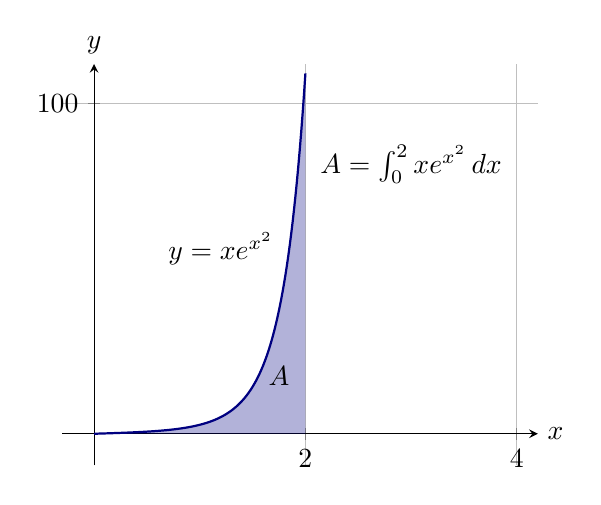
\begin{tikzpicture}
    \begin{axis}[
        xmin=-0.3,xmax=4.2,ymin=-0.3,ymax=3.5,
        clip=true,
        unit vector ratio*=2 2 2,
        axis lines=center,
        grid = major,
         width=3in,
        height=3in,
        ytick={0,3.125},
        xtick={0,2,4},
         yticklabels={0,100},
        xlabel=$x$, ylabel=$y$,
        every axis y label/.style={at=(current axis.above origin),anchor=south},
        every axis x label/.style={at=(current axis.right of origin),anchor=west},
      ]
     \addplot[fill=penColor,fill opacity=0.3,draw=none,domain=0:{2},samples=50]  {((1/32)*x*e^(x^2)} \closedcycle;;   
      \addplot[thick,penColor,domain=0:{2},samples=150] {((1/32)*x*e^(x^2)};   
  % \addplot [draw=none,fill=fillp,domain=8:9, smooth] {f(x)} \closedcycle;
	  \node at (axis cs:1.75,0.55) { $A$};  
	   \node at (axis cs:3,2.55) { $A=\int_0^2 xe^{x^2}\d x$};       
      \node at (axis cs:1.2,1.75) {$y=xe^{x^2}$};
      \end{axis}`
  \end{tikzpicture}
  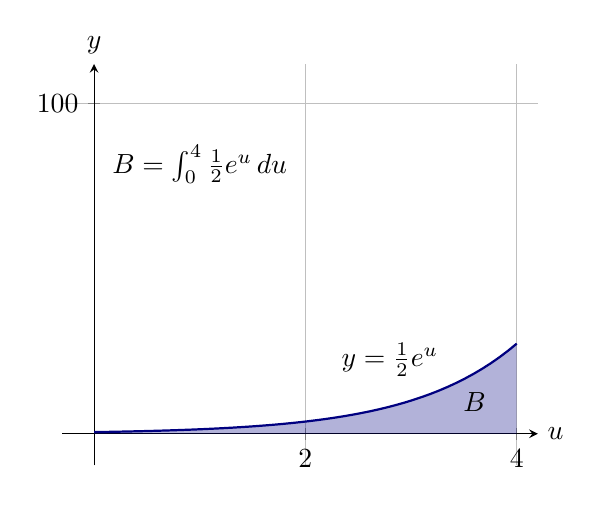
\begin{tikzpicture}
	  \begin{axis}[
        xmin=-0.3,xmax=4.2,ymin=-0.3,ymax=3.5,
        clip=true,
        unit vector ratio*=2 2 2,
        axis lines=center,
        grid = major,
         width=3in,
        height=3in,
        ytick={0,3.125},
        xtick={0,2,4},
         yticklabels={0,100},
        xlabel=$u$, ylabel=$y$,
        every axis y label/.style={at=(current axis.above origin),anchor=south},
        every axis x label/.style={at=(current axis.right of origin),anchor=west},
      ]
      \addplot[fill=penColor,fill opacity=0.3,draw=none,domain=0:{4},samples=50] {(1/64)*e^x} \closedcycle;
      \addplot[thick,draw=penColor,domain=0:{4},samples=50] {(1/64)*e^x};

	  \node at (axis cs:3.6,0.3) { $B$}; 
	   \node at (axis cs:1,2.55) {$B=\int_0^4 \frac{1}{2}e^{u}\d u$};           
      \node at (axis cs:2.8,0.7) {$y=\frac{1}{2}e^u$};
      \end{axis}`
  \end{tikzpicture}
\end{image}
The two shaded areas in the figure, $A= \int_0^2 x e^{x^2}\d x$ and $B=\frac{1}{2}\int_{0}^{4} e^{u}\d u$, appear to be equal,
and this confirms what was established by computation before.
  
  
Therefore, whenever we are faced with a problem of evaluating a difficult integral, we try to  replace it with  a simpler one, as long as  both  integrals represent the same net area.


\end{explanation}
\end{example}

We can solve a problem like this in a slightly different
way. Let's do the same example again, this time we will think in terms
of differentials.

\begin{example}\label{main example}
Compute:
\[
\int_0^2 x e^{x^2}\d x
\]
\begin{explanation}
Here we will set
\[ u=g(x) = x^2.
\]
 Then 
 \[
 \d u =g'(x)\d x=2x\d x.
 \]
Here, we are thinking in terms of differentials.
We can solve for $\d x$ to get 
\[
\d x = \frac{\d u}{2x}.
\]
Using this equality, we can write

\begin{align*}
\int_0^2 x e^{x^2}\d x &= \int_{g(0)}^{g(2)} x  e^{u} \frac{\d u}{2x}\\
  &= \int_{0}^{4} \frac{e^u}{2}\d u .
\end{align*}
At this point, we can continue as we did before and write
\[
 \int_{0}^{4} \frac{e^u}{2}\d u= \frac{\answer[given]{e^4} -e^0}{2}.
\]
\end{explanation}
\end{example}

Finally, sometimes we simply want to deal with the antiderivative on
its own.  We will repeat the example one more time in oder to demonstrate this approach.

\begin{example}
Compute:
\[
\int_0^2 x e^{x^2}\d x
\]
\begin{explanation}
We can apply the Second Fundamental Theorem of Calculus and, in order to do that, we first need to compute an indefinite integral.
\[
\int  x e^{x^2} \d x.
\]

As before, we set $u=g(x)=x^2$, and compute $\d u =  2x \d x$,
 thinking in terms of differentials. Now we see that
\[
\int   x e^{x^2} \d x = \int x e^{u} \frac{\d u}{2x} = \int \frac{e^{u}}{2}\d u .
\]
Hence 
\[
\int  x e^{x^2} \d x = \frac{e^{u}}{2}+C .
\]
This does not look right, since  we need to find an antiderivative of the function $ x e^{x^2},$ and our result is a function of $u$.
We can easily fix this, by simply substituting $u$ with $g(x)=x^2$.
Therefore,
\[
\int xe^{x^2}\d x =\frac{e^{u}}{2}+C= \frac{e^{x^2}}{2}+C .
\]
Finally, we can apply the SFTOC
\begin{align*}
\int_0^2 x e^{x^2}\d x &=\eval{\frac{e^{x^2}}{2}}_0^2\\
&= \frac{\answer[given]{e^4} -e^0}{2}.
\end{align*}
\end{explanation}
\end{example}

\section{More examples}

With some experience, it is (usually) not too hard to see what to
substitute as $u$.  We will work through the following examples in the
same way that we did for Example \ref{main example}.
\begin{example}
Compute:
\[
\int x^4(x^5+1)^{9} \d x
\]
\begin{explanation}
Here we set $u =  \answer[given]{x^5+1}$, so $\d u =  \answer[given]{5x^4} \d x$.  Then
it follows that $\d x=\frac{\d u}{5x^4}$. Therefore
\begin{align*}
  \int x^4(x^5+1)^{9} \d x &= \int x^4 (u)^{9} \frac{\d u}{5x^4} \\
  &= \frac{1}{5} \int u^{9} \d u\\
&=\frac{u^{10}}{ \answer[given]{50}}.
\end{align*}
Notice that this example is an indefinite integral and not a definite
integral, meaning that there are no limits of integration.  So we do
not need to worry about changing the endpoints of the integral.  However,
we do need to back-substitute into our answer, so that our final
answer is a function of $x$.  Recalling that $u= x^5+1$, we have
our final answer
\[
\int x^4(x^5+1)^{9} \d x= \frac{(x^5+1)^{10}}{\answer[given]{50}}+C.
\]
Reminder: you can always verify your result by differentiating.

\end{explanation}
\end{example}


If substitution works to solve an integral (and that is not always the
case!), a common trick to find what to substitute for is to locate the
``ugly'' part of the function being integrated.  We then substitute
for the ``inside'' of this ugly part.  While this technique is
certainly not rigorous, it can prove to be very helpful.  This is
especially true for students new to the technique of substitution.
The next two problems are really good examples of this philosophy.

\begin{example}
Compute:
\[
\int_{-1}^0 12x^3 \cos({x^4}) \d x
\]
\begin{explanation}
The ``ugly'' part of the function being integrated is $\cos({x^4})$.  The
``inside'' of this term is then $x^4$.  So a good possibility is to
try
\[
u =g(x)= x^4.
\]
Then
\[
\d u = (4x^3) \d x 	\qquad	\Rightarrow	\qquad	\d x = \answer[given]{\frac{1}{4x^3}} \d u
\]
and so
\begin{align*}
\int_{-1}^0 12x^3 \cos({x^4}) \d x &= \int_{g(-1)}^{g(0)} 12 x^3 \cos({u}) \answer[given]{\frac{1}{4x^3}} \d u  \\
&= \int_{\answer[given]{1}}^{\answer[given]{0}} 3 \cos({u}) \d u  \\
&= \eval{3\sin({u})}_{\answer[given]{1}}^{\answer[given]{0}}  \\
&= \answer[given]{3(0-\sin({1}))}.
\end{align*}
\end{explanation}
\end{example}




\begin{example}
  Compute:
  \[
  \int_{1}^{e^{\frac{\pi}{4}}} \frac{\cos(\ln x)}{x} \d x
  \]
\begin{explanation}
Here the ``ugly'' part here is $\cos(\ln x)$.  So we substitute for
the inside:
\[
u=g(x)=\answer[given]{\ln x}.
\]
Then
\[
\d u =  \answer[given]{\frac{1}{x}} \d x 	\qquad	\Rightarrow	\qquad	\d x = \answer[given]{x} \d u.
\]
Notice that
\begin{align*}
g(1) &= \ln (1) = \answer[given]{0} \\
g \left( e^{\frac{\pi}{4}} \right) &= \ln \left( e^{\frac{\pi}{4}} \right) = \answer[given]{\frac{\pi}{4}}.
\end{align*}
Then we substitute back into the original integral and solve:
\begin{align*}
\int_{1}^{e^{\frac{\pi}{4}}} \frac{\cos(\ln x)}{x} \d x &= \int_0^{\frac{\pi}{4}} \frac{\cos(u)}{x} x \d u  \\
&= \int_0^{\frac{\pi}{4}} \cos(u) \d u  \\
&= \eval{\answer[given]{\sin(u)}}_{0}^{\frac{\pi}{4}}  \\
&= \frac{\sqrt{2}}{\answer[given]{2}} - \answer[given]{0} = \frac{\sqrt{2}}{\answer[given]{2}}.
\end{align*}
\end{explanation}
\end{example}

To summarize, if we suspect that a given function is the derivative of
another via the chain rule, we introduce a new variable $u=g(x)$, where $g$ is a likely candidate for
the inner function. We rewrite the integral
 entirely in terms of $u$, with no $x$ remaining in the
expression. If we can integrate this new function of $u$, then the
antiderivative of the original function is obtained by replacing $u$
by $g(x)$.


\end{document}
